\documentclass{article}
\usepackage{graphicx} % Required for inserting images
\usepackage{graphicx} % Required for inserting images
%\usepackage[left=0.5in, right=0.5in, top=0.5in, bottom=0.5in]{geometry}
%\usepackage[left=1.5cm, right=1cm, top=0.5cm, bottom=1.5cm]{geometry}
\usepackage[left=1.5cm, right=1.5cm, top=0.5cm, bottom=1.5cm]{geometry}
\usepackage{amsmath}
\usepackage{amssymb}
\usepackage{amsfonts}
\usepackage{amsthm}
\usepackage{ulem}
\usepackage{bm}
\usepackage{tikz}
\usepackage{enumitem}

\date{}

\begin{document}
\fontsize{13}{15} \selectfont %This is 13pt text with 15pt line spacing.

\begin{center}
 \text{Potterhouse School. \hspace{1cm} Year 6 Math - Khadija (i).} \qquad \\ 
\end{center} \\ 

Name: ...........................................................  \hspace{0.5cm}  Date: ....................... \hspace{0.5cm}  Class: ......\hspace{0.5cm} %[20 marks]

\par
\vspace*{5pt} 
\textit{(You must show your working including the times tables of the divisors and multipliers.)  }
%\vspace{5pt}

% \begin{center}
  %  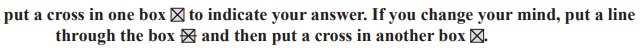
\includegraphics[width=15cm]{Year_6_Mixed_Tests/Xx.png}
% \end{center}
% \\

\begin{enumerate}
     
 \item \quad Evaluate: \( 4 + 2^{2} \div (3 + 1 ) \) % \hspace {2cm} [1 mark]
\vspace{10pt}
%\hline
\vspace{5pt}

\item \quad A factory bakes 3457 cakes and packs them in containers with 24 cakes in each container.  \\
\quad (a) How many containers are needed? \\
\quad (b) How many cakes will remain? 
%\vspace{120pt}
%\hline
\vspace{10pt}
% \hline
\vspace{5pt}


\item \quad Write these numbers in order of size. Start with the smallest. %\\
\begin{center}
5.75 \hspace{2cm} 5.705  \hspace{2cm} 57.5 \hspace{2cm} 570.05 \hspace{2cm} 5.075 
\end{center}
%\vspace{5pt}

 %..... \hspace{3cm} ..... \hspace{3cm}  ..... \hspace{3cm} ..... \hspace{3cm} .....  

%\par
%\text{smallest} 
\vspace{10pt}
% \hline
\vspace{5pt}

\item \quad Write these numbers in order of size. Start with the smallest. %\\
\begin{center}
0.403 \hspace{2cm} 0.043 \hspace{2cm} 43\% \hspace{2cm}  \( \displaystyle \frac{3}{4} \) 
\end{center}
%\vspace{70pt}

 %..... \hspace{3cm} ..... \hspace{3cm}  ..... \hspace{3cm} .....     \\

 %smallest
 
 %\begin{flushright}
 %   \text{(2)}
%\end{flushright}
 
 \vspace{10pt}
 %\hline
 \vspace{5pt}

\item \quad Fill in A, B, C and D in the number line below.  %\hspace{2cm} [2 marks]
\vspace{10pt}

\begin{tikzpicture}[x=0.8cm]  % Set the x unit vector length to 0.8cm
    % Draw the main line
    \draw[->] (-10,0) -- (10,0);
    
    % Draw tick marks and labels
    \foreach \x in {-10, -8, ..., 10} {
        \draw (\x,-0.1) -- (\x,0.1);
        % Omit labels at positions -7, -3, 2, and 8 to leave them blank for letters
        \ifnum\x=-8 \else \ifnum\x=-6 \else \ifnum\x=-2 \else 
        \ifnum\x=2 \else \ifnum\x=4 \else  \ifnum\x=8 \else 
            \node[below] at (\x,-0.2) {$\x$};
        \fi\fi\fi\fi\fi\fi
    }
    
    % Draw letters 'A', 'B', 'C', and 'D' at positions -7, -3, 2, and 8
    \node[below] at (-8,-0.2) {A};
    \node[below] at (-6,-0.2) {B};
    \node[below] at (-2,-0.2) {C};
    \node[below] at (2,-0.2) {D};
    \node[below] at (4,-0.2) {E};
    \node[below] at (8,-0.2) {F};
   % \node[below] at (8,-0.2) {D};
    
\end{tikzpicture}
\vspace{10pt}

 %\hline
 \vspace{5pt}

\item \quad Add. % \hspace{2cm} [2 marks]
\[
\begin{array}{cccccc}
& 7 & 8 & 2 & 0 & 1 \\
  & & 3 & 6 & 9 & 8 \\
+ & & & 2 & 7 & 1 \\
\hline
&  &  &  &  &  \\
\\ 
\hline 
\end{array}
\]

\vspace{10pt}
 %\hline
 \vspace{5pt}

\item \quad Lay out and solve: \hspace{2cm} 45001 - 3997 %\hspace{2cm} [2 marks]
\vspace{10pt}

 %\hline
 \vspace{5pt}

 \item \quad Make the fractions equivalent: $$ \displaystyle\frac{2}{7} = 
\genfrac{}{}{1pt}{0}{\fbox{\makebox[1em]{\rule{0pt}{1em}}}}{21} $$
\vspace{10pt}

\item \quad Simplify: \(  \displaystyle \frac{18}{24} \)
\vspace{10pt}

\item \quad Convert the mixed number to an improper fraction: \(  \displaystyle 4 \frac{3}{7} \) \\

% \raggedleft (2 marks)

\end{enumerate}

 \end{document}